\documentclass{article}

\usepackage[nolist,nohyperlinks]{acronym}
\usepackage{amsmath,amsfonts,amssymb}
\usepackage{subfig}
\usepackage{graphicx}

%%%%%%%%%%%%%%%%%%% Acronyms definitions %%%%%%%%%%%%%%%%%%%%%

\begin{acronym}
\acro{LNS}{Large Neighborhood Search}
\acro{RS}{Random Search}
\end{acronym}

\begin{document}
\section*{Relax Rate Selection}
\label{sec:relax_rate_selection}

In \ac{LNS}, the relax rate, $r$, affects
how many of the variables of the last solution
\ac{LNS} destroys for finding the next solution.
To evaluate that, we use two metrics, $P_{\delta}$ and $P_{t}$
that correspond to the rate of the \ac{LNS} over \ac{RS} with regards
to the pairwise distance and the diversification time as follows:

\begin{equation}
  P_{\delta}(\delta, S_1, S_2) = \begin{cases}
    \displaystyle \frac{d(\delta, S_1)}{d(\delta, S_2)},& d(\delta, S_1) > d(\delta, S_2) \\
    \displaystyle \frac{d(\delta, S_2)}{d(\delta, S_1)},& otherwise
    \end{cases}
    \label{eq:impr}
\end{equation}

\noindent
and

\begin{equation}
  P_{t}(t_1, t_2) = \begin{cases}
    \displaystyle \frac{t_1}{t_2},& t_1> t_2\\
    \displaystyle \frac{t_2}{t_1},& otherwise
    \end{cases}
    \label{eq:imprt}
\end{equation}

\noindent
where, $t_1$ is the diversification time for generating the solution set $S_1$ for \ac{RS}
and $t_2$ is the diversification time for generating the solution set $S_2$ for \ac{LNS}.

\begin{figure}[h!]
  \centering
  \subfloat[\label{fig:reldist}Diversity improvement]{
    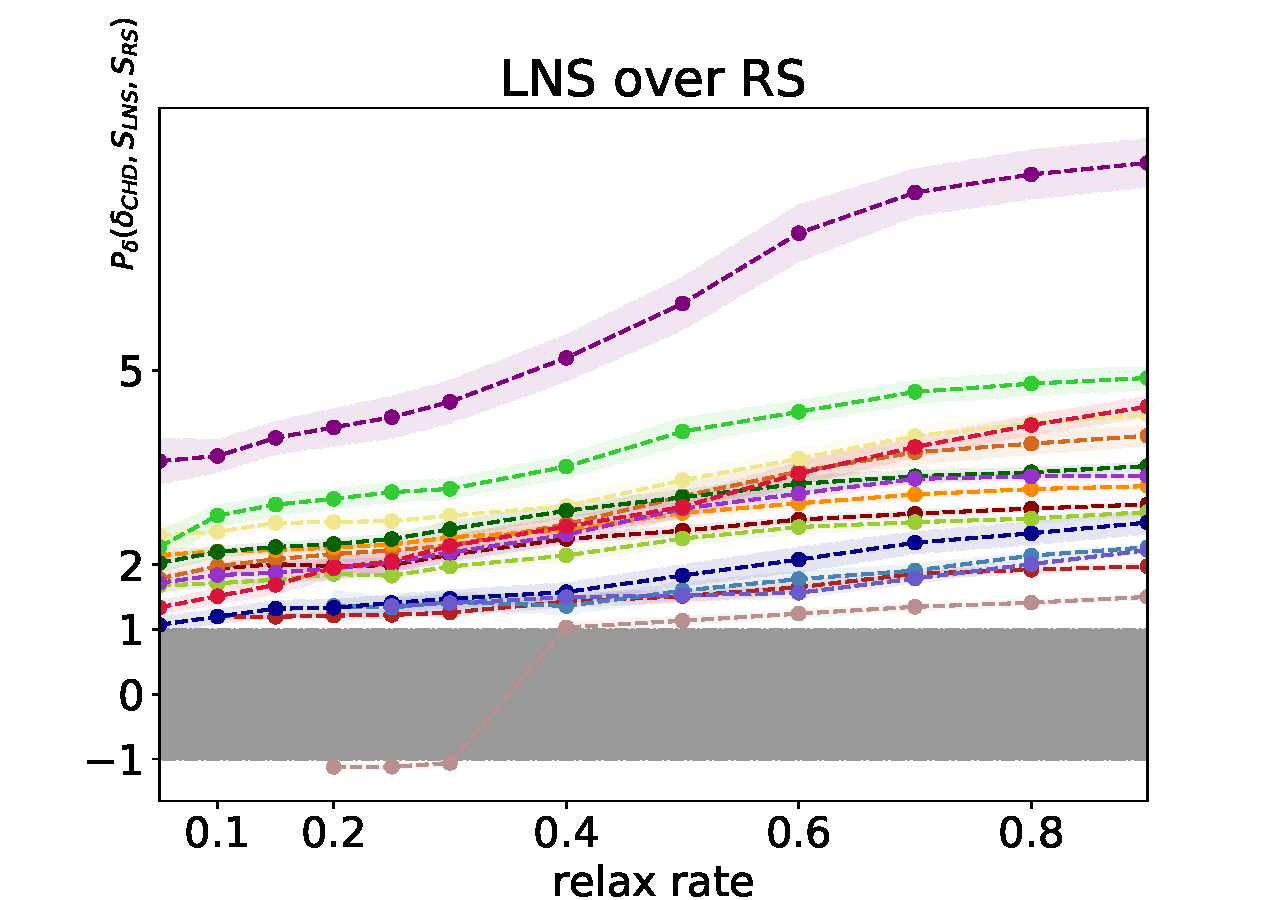
\includegraphics[trim={1.5cm 0cm 2cm 0cm}, clip, width=0.45\textwidth]{figs/lns_vs_rs_dist_hamming.pdf}
  }
  \subfloat[\label{fig:reltime} Diversification time improvement]{
    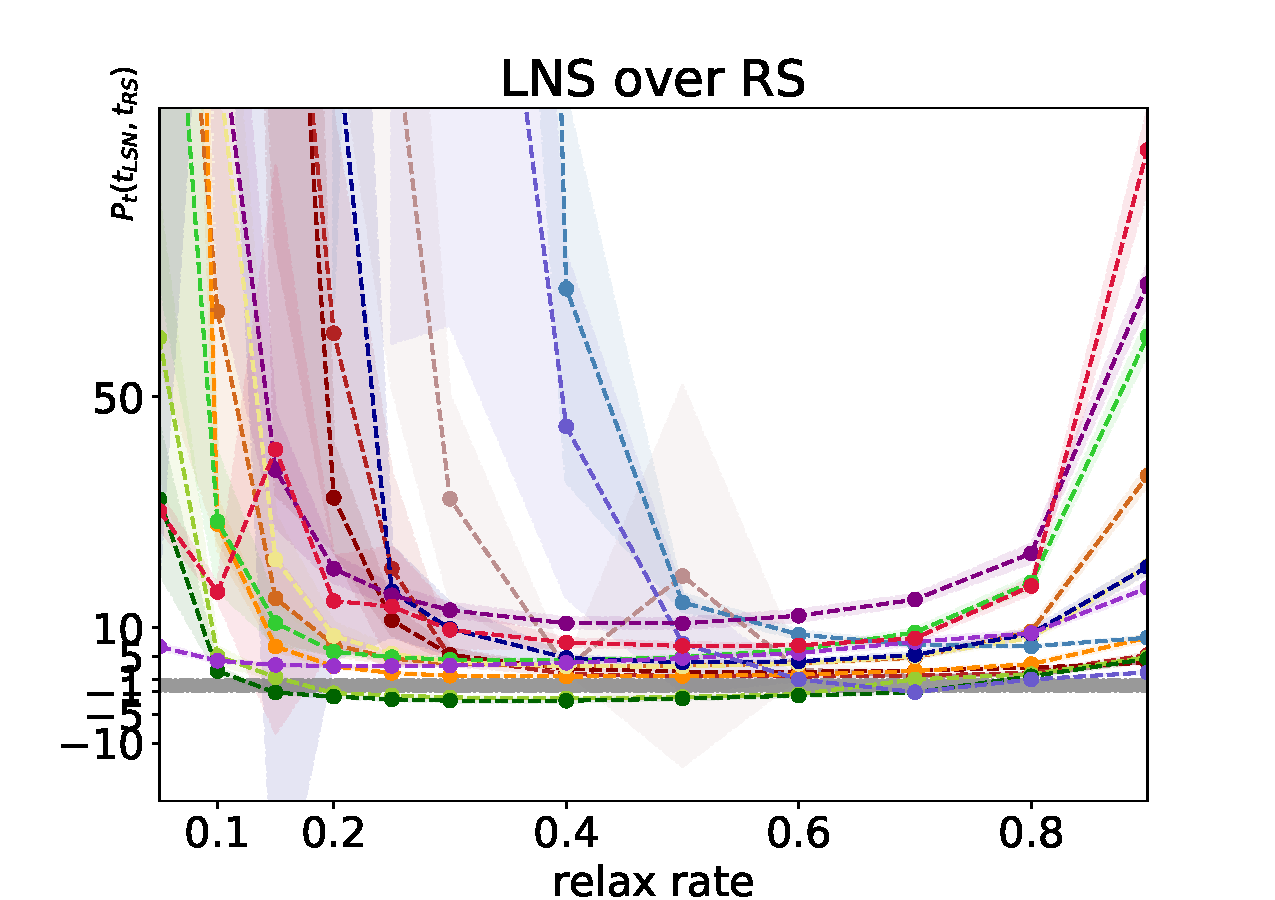
\includegraphics[trim={1.5cm 0cm 2cm 0cm}, clip, width=0.45\textwidth]{figs/lns_vs_rs_time_hamming.pdf}
  }
  \caption{\label{fig:relax} Improvement 
    in diversity and diversification
    time of \ac{LNS} over \ac{RS} for different values of the relax rate }
\end{figure}


Figure~\ref{fig:relax} depicts the effect of different relax rates on
the distance, $\delta_{HD}$ and the solving time for generating 200 variants.
The Figure shows that increasing the relax rate increases
the pair-wise distance, $d$ (Equation~\ref{eq:aggr}), of the generated program variants. 
The diversifying time (Figure~\ref{fig:reltime}), however, has a different form.
Figure~\ref{fig:reltime} shows that low values and large values of $r$ have
large time overhead, whereas values $r=0.6$ and $r=0.7$ have less time overhead.
For this reason, the evaluation uses $r=0.7$ that corresponds to both low time overhead and
high distance improvement.
\end{document}
